\chapter{Problematika digitální stopy\\ ve školách}

Praktická část této balakářské práce se zabývá navržením a vytvořením prostředí (\textit{aplikace}) pro vzdělávání v~této tématice.
Je rozdělena do dvou kapitol. První kapitola popisuje východiska aplikace, druhá pak její technický návrh a řešení.

\section{Zařazení problematiky digitální stopy do školních výukových materiálů}

První oblastí východisek je zařazení tématu osobních dat a digitální stopy do kontextu vzdělávacích materiálů.
Zaměřuje se na to, jakou roli a prostor v~nich aktuálně (v~kontextu narůstající důležitosti tématu ve společnosti a společenských debatách) zaujímá.

\subsection*{Vymezení pojmů}

Pro snazší orientaci v~kapitole zde shrnuji použité zkratky a kódy a jejich význam:

\textbf{RVP} -- Rámcový vzdělávací program:

\begin{displayquote}
\uv{Rámcové vzdělávací programy (RVP) tvoří obecně závazný rámec pro tvorbu školních vzdělávacích programů škol všech oborů vzdělání v~předškolním, základním, základním uměleckém, jazykovém a středním vzdělávání. Do vzdělávání v~České republice byly zavedeny zákonem č. 561/2004 Sb., o~předškolním, základním, středním, vyšším odborném a jiném vzdělávání (školský zákon).} \citep{rvp} 
\end{displayquote}

\textbf{Klasifikace SŠ}:

\textbf{Obory s~maturitou}

\textbf{SŠ (M)} -- úplné střední odborné vzdělání s~maturitou (obory kategorie M)

\begin{displayquote}
\uv{příprava má profesní charakter a délka studia je 4 roky. Po maturitě lze pokračovat ve vzdělávání na vysoké nebo vyšší odborné škole.} \citep{stredni-vzdelavani}
\end{displayquote}

\textbf{SŠ (L)} -- úplné střední odborné vzdělání s~odborným výcvikem a maturitou (obory kategorie L)

\begin{displayquote}
\uv{studium připravuje pro náročná dělnická povolání a nižší řídicí funkce. V~denní formě je 4leté a jeho významnou součástí je odborný výcvik (obory vznikly z~dřívějších 3letých učebních oborů). Absolventi získávají maturitní vysvědčení a mohou pokračovat ve vzdělávání na vysoké nebo vyšší odborné škole.} \citep{stredni-vzdelavani}
\end{displayquote}

\textbf{SŠ (K)} -- úplné střední všeobecné vzdělání (obory kategorie K)

\begin{displayquote}
\uv{všeobecná příprava ve 4letých a víceletých gymnáziích je neprofesní a připravuje především pro vysokoškolské nebo vyšší odborné vzdělávání.} \citep{stredni-vzdelavani}
\end{displayquote}

\textbf{Obory s~výučním listem}

\textbf{SŠ (H)} -- střední odborné vzdělání s~výučním listem (obory kategorie H)

\begin{displayquote}
\uv{tradiční učební obory s~tříletou přípravou ve středních odborných učilištích. Po získání výučního listu lze pokračovat navazujícím nástavbovým studiem a získat i maturitu.} \citep{stredni-vzdelavani}
\end{displayquote}

\textbf{SŠ (E)} -- nižší střední odborné vzdělání (obory kategorie E)

\begin{displayquote}
\uv{studium je tříleté nebo dvouleté, výstupem je výuční list. Obory mají nižší nároky v~oblasti všeobecného i obecně odborného vzdělání a jsou určeny především pro žáky se speciálními vzdělávacími potřebami, např. pro absolventy dřívějších speciálních základních škol a žáky, kteří ukončili povinnou školní docházku v~nižším než 9. ročníku základní školy. Obory připravují pro výkon jednoduchých prací v~rámci dělnických povolání a ve službách.} \citep{stredni-vzdelavani}
\end{displayquote}

\subsection{Vymezení dokumentů}

Pro prozkoumání, jak jsou témata zařazena ve vzdělání, budou primárním zdrojem RVP. Je nutné se dívat na jejich návaznost, podobnosti a rozdíly na různých stupních a zaměřeních vzdělávání.

Konkrétně tedy budou prozkoumány RVP pro základní vzdělávání, které definují vzdělávací oblast Informatiky a její cíle, a dále RVP pro gymnázia a vybrané odborné školy se zaměřením na Informatiku a Informační technologie. 

Kromě toho budou rozebrány aktuální plány na revizi oblasti Informatiky a ICT, která může přinášet změny i v~této oblasti, a zároveň ukazovat na možné trendy v~pojetí vzdělávání v~oblasti digitálního světa a technologií a s~tím souvisejících témat.

Konkrétně tedy kapitola prozkoumá propojení na následující dokumenty:

\begin{itemize}
\item Rámcové vzdělávací programy
	\begin{itemize}
    \item RVP základní školy \citep{rvp-zs}
    \item RVP-G (kategorie L) \citep{rvp-g}
    \item RVP pro odborné školy -- Informační technologie \citep{rvp-it} (kategorie M)
    \item RVP pro odborné školy -- Informační služby\citep{rvp-is} (kategorie M)
	\end{itemize}
\item Návrh revizí rámcových vzdělávacích programů v oblasti informatiky a informačních a komunikačních technologií \citep{revize}
\end{itemize}

\subsection{Rámcové vzdělávací programy}

\subsubsection*{RVP základní školy}

\textbf{Vzdělávací oblast Informatika}

Ve vymezení Cílového zaměření vzdělávací oblasti je v~kontextu tématu důležitý tento bod:

\begin{displayquote}
	\uv{uvědomění si, respektování a zmírnění negativních vlivů moderních informačních a komunikačních technologií na společnost a na zdraví člověka, ke znalosti způsobů prevence a ochrany před zneužitím a omezováním osobní svobody člověka}
	\citep{rvp-zs},
\end{displayquote}

konkrétně však tento bod není vymezen cíli ani učivem, které by s~oblastí osobních dat a digitální stopy přímo souviselo.

\subsubsection*{RVP-G}

\textbf{Vzdělávací oblast Informatika a informační a komunikační technologie}

Vzdělávací oblast Informatika a informační a komunikační technologie v~RVP pro vyšší stupně vzdělávání navazuje na obast Informatika v~RVP pro základní školy. V~cílovém zaměření vzdělávací oblasti se tedy nachází totožný bod:

\begin{displayquote}
	\uv{uvědomění si, respektování a zmírnění negativních vlivů moderních informačních a komunikačních technologií na společnost a na zdraví člověka, ke znalosti způsobů prevence a ochrany před zneužitím a omezováním osobní svobody člověka}
	\citep{rvp-g}
\end{displayquote}

V~oblasti Zdroje a vyhledávání informací, Komunikace je v~učivu bod:

\begin{displayquote}
	\uv{informační etika, legislativa – ochrana autorských práv a osobních údajů}
	\citep{rvp-g},
\end{displayquote}

navazující na výstup

\begin{displayquote}
	\uv{využívá informační a komunikační služby v~souladu s~etickými, bezpečnostními a legislativními požadavky}
	\citep{rvp-g}.
\end{displayquote}

Alespoň částečně tedy jde o~problematiku osobních údajů, ačkoli více z~pohledu legislativního a etického než z~pohledu soukromí.

V~dalších oblastech se pak téma neobjevuje. 

\subsubsection*{RVP odborné školy -- Informační technologie}

V~cílech vzdělávání můžeme najít následující body:

\begin{displayquote}
	\uv{\textbf{neohrožovali svým chováním v~digitálním prostředí sebe, druhé}, ani technologie samotné}
	\citep{rvp-it},
\end{displayquote}

\begin{displayquote}
	\uv{\textbf{uvědomovali si, že technologie ovlivňují společnost, a naopak chápali svou odpovědnost při používání technologií}}
	\citep{rvp-it}.
\end{displayquote}

Ve výsledcích vzdělávání pak najdeme konkrétní body:

\begin{displayquote}
	\uv{\textbf{chrání} digitální zařízení, digitální obsah i \textbf{osobní údaje} v~digitálním prostředí před poškozením, přepisem/změnou či \textbf{zneužitím}; reaguje na změny v~technologiích ovlivňujících bezpečnost}
	\citep{rvp-it},
\end{displayquote}

\begin{displayquote}
	\uv{s~vědomím souvislostí fyzického a digitálního světa \textbf{vytváří a spravuje jednu či více digitálních identit; kontroluje svou digitální stopu, ať už ji vytváří sám nebo někdo jiný, v~případě potřeby dokáže používat služby internetu anonymně}}
	\citep{rvp-it}.
\end{displayquote}

\subsubsection*{RVP odborné školy -- Informační služby}

V~tomto RVP se žádné body přímo související s~tématikou nenachází.

\subsection{Návrh revizí RVP v~oblasti Informatiky a informačních a komunikačních technologií}

Aktuálně se pracuje na revizi RVP v~oblasti Informatiky a informačních a komunikačních technologií, je tedy vhodné se podívat, zda tato revize nějak mění zakotvení tématu digitální stopy a osobních dat ve vzdělávání.

Jedno ze základních východisek návrhu revize je rozvoj digitální gramotnosti, v~dokumentu definované jako:

\begin{displayquote}
	\uv{Digitální gramotností rozumíme soubor digitálních kompetencí (vědomostí, dovedností, postojů, hodnot), které jedinec potřebuje k bezpečnému, sebejistému, kritickému a tvořivému využívání digitálních technologií při práci, při učení, ve volném čase i při svém zapojení do společenského života.}
	\citep{revize},
\end{displayquote}

V~oblastech digitální gramotnosti může být pak pro naše téma relevantní bod:

\begin{displayquote}
	\uv{Vnímá a hodnotí potenciál i rizika zapojení digitálních technologií do různých procesů a v různých situacích a podle toho zodpovědně jedná.}
	\citep{revize}.
\end{displayquote}

Jak se to promítá přímo do očekávaných výstupů můžeme vidět v~tabulce níže:

\begin{figure}[h]
\centering
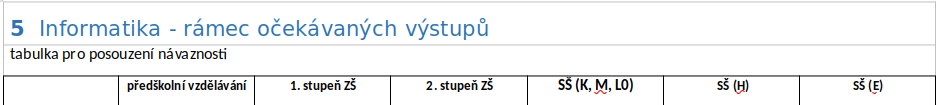
\includegraphics[width=\linewidth]{images/01_revize.png}
\end{figure}

\begin{figure}[h]
\centering
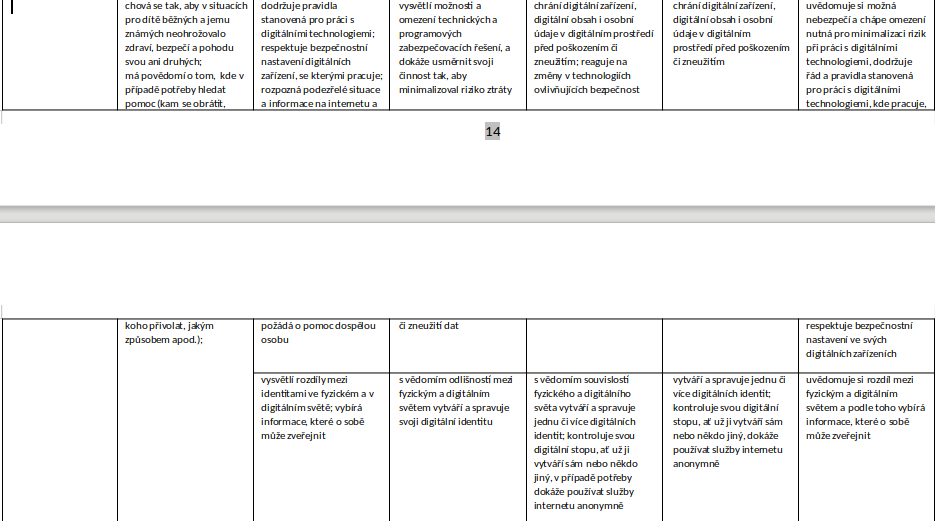
\includegraphics[width=\linewidth]{images/02_revize.png}
\end{figure}
\begin{figure}[h]
\centering
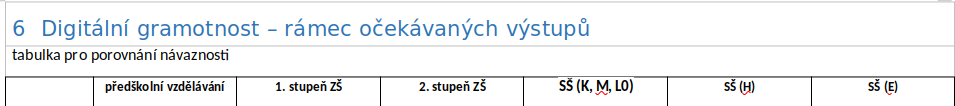
\includegraphics[width=\linewidth]{images/03_revize.png}
\end{figure}
\begin{figure}[h]
\centering
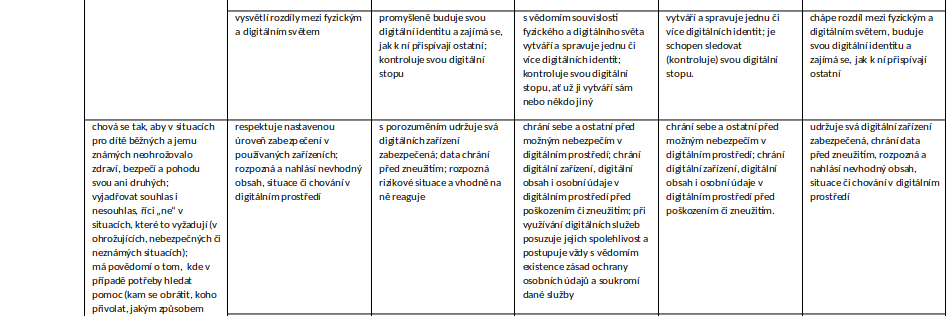
\includegraphics[width=\linewidth]{images/04_revize.png}
\end{figure}
\begin{figure}[h]
\centering
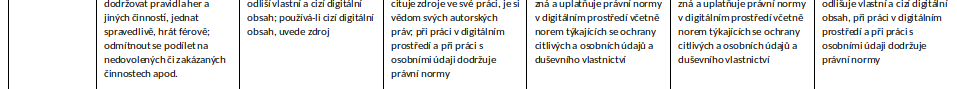
\includegraphics[width=\linewidth]{images/05_revize.png}
\end{figure}

\pagebreak
Na všech typech SŠ nacházíme výstup:

\begin{displayquote}
	\uv{\textbf{chrání} digitální zřízení, digitální obsah i \textbf{osobní údaje} v~digitálním prostředí před poškozením či zneužitím}
	\citep{revize}.
\end{displayquote}

A~pro školy v~kategoriích K, L, M, H dále

\begin{displayquote}
	\uv{\textbf{kontroluje} svou \textbf{digitální stopu}, ať už ji vytváří sám nebo někdo jiný, dokáže používat služby internetu anonymně}
	\citep{revize},
\end{displayquote}

a pro SŠ (E) podobný bod

\begin{displayquote}
	\uv{buduje svou digitální identitu a zajímá se, jak k~ní přispívají ostatní}
	\citep{revize}.
\end{displayquote}

\subsection*{Shrnutí}

Téma osobních dat a digitální stopy můžeme v~aktuálních vzdělávacích materiálech najít v~obecném vymezení v~cíli vzdělávací oblasti Informatika (respektive Informatika a informační a komunikační technologie) v~bodě:

\begin{displayquote}
	\uv{uvědomění si, respektování a zmírnění negativních vlivů moderních informačních a komunikačních technologií na společnost a na zdraví člověka, ke znalosti způsobů prevence a ochrany před zneužitím a omezováním osobní svobody člověka}
	\citep{rvp-g}.
\end{displayquote}

Konkrétní vzdělávací výsledky s~tímto tématem se nacházejí pouze u~RVP odborných škol oboru Informační technologie.

Zároveň se však toto téma výrazněji objevuje v~návrhu revize, a lze tedy předpokládat, že se do RVP (a následně ŠVP jednotlivých škol) bude více promítat.

Vznik materiálů a prostředí pro zařazení této problematiky do výuky je tedy možné považovat za užitečný a do budoucna nutný.



\section{Východiska pro tvorbu aplikace}
Jak vyplývá z~předchozí sekce, téma digitální stopy a osobních dat se nejspíše bude po revizích více objevovat v~RVP středních škol. Na tuto skupinu studentů tedy bude aplikace cílit.

Prostředí může sloužit jako součást většího vzdělávacího oblouku, ovšem tato práce si nedává za cíl vytvoření metodik pro učitele, a tedy musí obsah aplikace fungovat i sám o~sobě.

Cílem je uživatele (studenty) v~aplikaci seznámit s~tématem atraktivní formou.

Zároveň však součástí aplikace musí být kvalitní napojení na teorii i reálné příklady, včetně informování uživatele o~tom, jak může svou digitální stopu spravovat.

\subsection{Návrh aplikace z~pohledu uživatele}
Návrh aplikace je následující:\\
Uživatel má možnost odehrát jednotlivé \uv{Mise}, které představují fiktivní příběh. V~každé Misi má uživatel ze simulovaných osobních dat různého typu vyřešit na začátku danou otázku.
Zjednodušený use-case tedy je:
\begin{itemize}
	\item uživatel si vybírá Misi
	\item uživatel je seznámen s~příběhem Mise (symbolickým rámcem) a cílem - co je potřeba zjistit pro splnění Mise
	\item uživatel využívá dané datasety pro nalezení řešení
	\item po správném zadání odpovědi jsou uživateli zobrazeny doplňující informace - napojení na teorii, příklady z~reálného světa, možnosti zabezpečení se v~podobné situaci.
\end{itemize}

Všechny akce (například přihlašování) probíhají pouze v~rámci aplikace na fiktivních datech, ač simulují reálné digitální služby.

V~sekci \textit{Scénáře} budou popsány konkrétní možné scénáře, z~nich část bude použita v~prototypu.

\subsection{Prototyp}
Jak bylo řečeno, součástí práce je vytvoření prototypu. Ten tedy nemusí mít všechny funkce či grafické řešení aplikace, která by byla reálně veřejně použita ve vzdělávání, má za cíl pouze najít vhodnou podobu, otestovat její technickou proveditelnost a náročnost a získat zpětnou vazbu od vybraných testerů.


\subsection{Scénáře}
Jak bylo popsáno, jádrem aplikace jsou Mise - tedy jednotlivé příběhy, ve kterých se uživatel seznamuje s~různými situacemi, týkajícími se osobních dat.

Aplikace bude navržena tak, aby bylo možné snadno další scénáře přidávat a tím rozšiřovat její vzdělávací potenciál (například v~zacílení na jiné věkové skupiny).

Scénáře vycházejí z~dat a rizik popsaných v~předchozích kapitolách, a cílí na různé typy a kategorie dat.


\subsubsection*{Odhadnutí hesla}
\textbf{Cíl}\\
Uhodnout heslo blízké osoby na sociální síť.\\
\textbf{Používané zdroje dat}\\
Příspěvky na sociální síti.\\
\textbf{Typ dat}\\
Veřejné / veřejné pro okruh lidí.\\
\textbf{Dodatečné informace}\\
Informace o~tom, jak lidé tvoří hesla\\
Případy toho, kdy lidé měli veřejně informace, jež vedly k~prolomení hesla\\
Obecná doporučení, jak chránit svoje hesla\\
Upozornění na nelegálnost takové činnosti v~reálním životě\\

V~tomto scénáři je úkolem uhodnout heslo do sociální sítě. Scénář se odkazuje na témata vhodného zabezpečení svých účtů a situací, kdy uživatelem sdílené informace napomáhají k~prolomení jeho obran.

Jde o~jednoduchý scénář vhodný pro seznámení s~aplikací. Je cíleně zjednodušený oproti realitě a pracuje s~veřejnými daty z~jednoho zdroje.

\textit{Scénář se nezabývá hesly z~pohledu kryptografického a obecně bezpečnostního, neboť to je již mimo rozsah naší práce. Bylo by však pravděpodobně možné takový scénář do aplikace přidat pro vzdělávání v~této oblasti.}


\subsubsection*{Plánování vloupání}
\textbf{Cíl}\\
Naplánovat vloupání do domu dané osoby -- udělat si představu o~jejím bydlišti a době, kdy bude dům prázdný.\\
\textbf{Používané zdroje dat}\\
Příspěvky na sociální síti\\
Příspěvky z~fitness sociální sítě\\
Stránky firmy\\
\textbf{Typ dat}\\
Veřejná data\\
\textbf{Dodatečné informace}\\
Případy z~praxe\\
Obecná doporučení, jak se tomuto typu útoku bránit\\ 
Upozornění na nelegálnost takové činnosti v~reálním životě\\

Tento scénář již ukazuje práci s~více zdroji dat a klade na uživatele větší nároky v~hledání částí informací.


\subsubsection*{Vyšetřování korupce}
\textbf{Cíl}\\
U~podezřelé osoby vyšetřit možné korupční vazby na jiné osoby.\\
\textbf{Používané zdroje dat}\\
Lokační data od operátorů\\
Výpisy z~bankovního účtu\\
Výpisy hovorů a SMS zpráv\\
\textbf{Typ dat}\\
Soukromé -- dostupné pouze poskytovatelům a v~oprávněných případech policii\\
\textbf{Dodatečné informace}\\
Informace o~sběru a uchovávání dat operátory\\
Informace o~přesnosti lokačních dat\\
Informace o~právních možnostech policie si tato data vyžádat\\


\subsubsection*{Výběr vhodné reklamy} 
\textbf{Cíl}\\
Vybrat, jaké reklamy zobrazit jakým uživatelům.\\
\textbf{Používané zdroje dat}\\
Příspěvky na sociálních sítích\\
Chování na sociálních sítích\\
Historie prohlížení\\
Lokační data\\
\textbf{Typ dat}\\
Soukromé -- data sbírají aplikace.\\
\textbf{Dodatečné informace}\\
Napojení na teorii \textit{attention economy}\\
Informace o~možnostech nastavení ochrany soukromí v~různých aplikacích.\\

Tento scénář simuluje fungování vyhodnocování dat algoritmy firem, jako je Facebook nebo Google, a následnou reklamní aukci. Má potenciál, aby na něj bylo navázáno šířeji tématem personalizované reklamy a \textit{attention economy}. 


Některé scénáře ukazují činnost, jež je ilegální. Motivací pro jejich zachování je to, že  možnost prožít si situaci z~pohledu útočníka může vést k~lepšímu prožití a přenesení do uvažování o~vlastní ochraně. Zároveň u~každého takového scénáře bude upozorněno, že jde o~simulaci -- akce probíhá pouze v~rámci této aplikace, a veškerá použitá data jsou fiktivní -- a jaké trestněprávní dopady by taková činnost měla v~reálném světě.

Scénáře vyjmenované v~této sekci jsou pouze příkladem možných scénářů použitých v~aplikaci. Nepředstavují všechny typy dat, a je pravděpodobné, že aplikace bude i po zveřejnění rozšiřována o~další.


\section*{Shrnutí}
Tato kapitola představila východiska pro tvorbu aplikace a propojila dosud získané poznatky z~této oblasti s~potřebami školství.  